
\begin{equation}
    [G]~[v(t)] = [i(t)]-[I_{hist}]
\end{equation}

\subsection{Line models}
\subsubsection{Bergeron's lossless line model}

\begin{figure}[H]
  \centering
  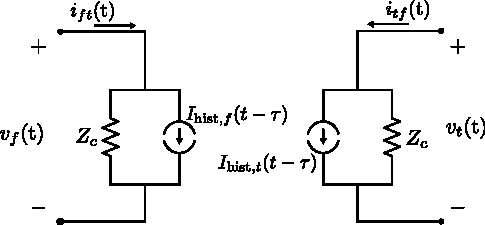
\includegraphics[width=0.6\linewidth]{inkscape_svg/bergeron_lossless.pdf}
  \caption{Bergeron's lossless line model.}
  \label{fig:bergeron_lossless}
\end{figure}

\begin{equation}
    i_{f,t}(t) = \frac{1}{Z_c}v_f(t)+I_{hist,f}(t-\tau)
\end{equation}
\begin{equation}
    i_{t,f}(t) = \frac{1}{Z_c}v_t(t)+I_{hist,t}(t-\tau)
\end{equation}

\begin{equation}
    I_{hist,f}(t-\tau) = -\frac{1}{Z_c}v_t(t-\tau)-i_{t,f}(t-\tau)
\end{equation}

\begin{equation}
    I_{hist,t}(t-\tau) = -\frac{1}{Z_c}v_f(t-\tau)-i_{f,t}(t-\tau)
\end{equation}

\begin{equation}
    Z_c = \sqrt{L'/C'}
\end{equation}

\begin{equation}
    v = \frac{1}{\sqrt{L'/C'}}
\end{equation}

\subsubsection{Bergeron's line model with lumped resistance}

\begin{figure}[H]
  \centering
  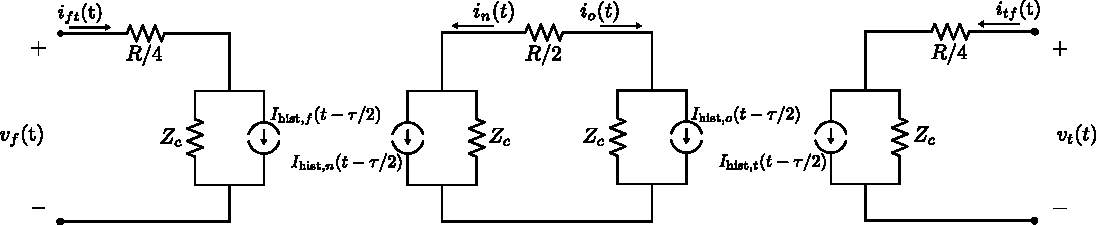
\includegraphics[width=1\linewidth]{inkscape_svg/bergeron_with_losses_full.pdf}
  \caption{Bergeron's line model with lumped resistance.}
  \label{fig:bergeron_losses}
\end{figure}

\begin{equation}
    Z = Z_c + R/4
\end{equation}

\begin{equation}
    H = \frac{Z_c - R/4}{Z_c + R/4}
\end{equation}


\begin{figure}[H]
  \centering
  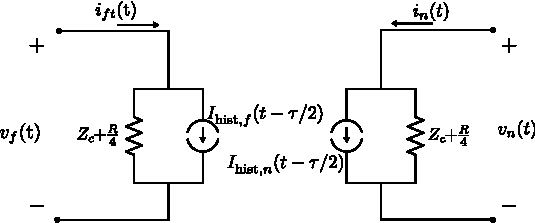
\includegraphics[width=0.6\linewidth]{inkscape_svg/bergeron_half_line_losses.pdf}
  \caption{Half Bergeron's line model with lumped resistance.}
  \label{fig:bergeron_losses_half}
\end{figure}

\begin{equation}
    I_{\text{hist},k}(t-\tau/2) = \frac{-1}{Z_c+R/4}v_m(t-\tau/2)- H~i_m(t-\tau/2)
\end{equation}

\begin{figure}[H]
  \centering
  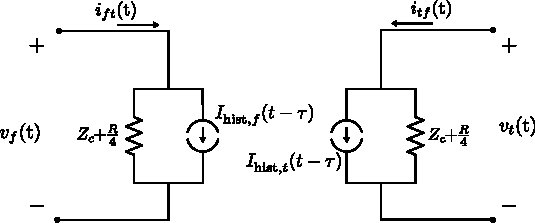
\includegraphics[width=0.6\linewidth]{inkscape_svg/bergeron_losses_equivalent.pdf}
  \caption{Bergeron's line model with lumped resistance two nodes equivalent.}
  \label{fig:bergeron_losses_equiv}
\end{figure}


\begin{equation}
    I_{hist,f}(t-\tau) = (\frac{1+H}{2})~(\frac{-1}{Z}v_t(t-\tau)-i_{t,f}(t-\tau)) + \\
    (\frac{1-H}{2})~(\frac{-1}{Z}v_f(t-\tau)-i_{f,t}(t-\tau))
\end{equation}

\begin{equation}
    I_{hist,t}(t-\tau) = (\frac{1+H}{2})~(\frac{-1}{Z}v_f(t-\tau)-i_{t,t}(t-\tau)) + \\
    (\frac{1-H}{2})~(\frac{-1}{Z}v_t(t-\tau)-i_{t,f}(t-\tau))
\end{equation}






idea de com funcionar:

- tot numèric. per cada element es crea numèricament la seva pròpia G i Itotal=Isource-Ihist i després s'uneix
tot a la G i Itotal gran del sistema. 

- es fa distinció entre elements actius(generador, etc) i passius (línies, trafos...)

- Els elements actius tindran les seves equacions internes definides simbòlicament i es podran resoldre a cada timestep.
aquests tindran la tensió com a input i les iabc com a output. També d'aquest model s'ha de poder arribar al Norton equivalent:
Req i isource eq tenint en compte que les equacions internes poden ser molt diferents entre elles.

- El sistema de simulació EMT no té per a res el mateix format que RMS i no seguirà el format de blocs de RMS.

- G només canvia si hi ha events, en canvi Itotal canvia a cada pas de temps.

- S'inicialitza el sistema a 0 (s'engega tot) i quan ja està a steady state es conta tau i d'allà es pot començar a contar t=0 en endavant.

- els paràmetres/constants de cada element s'han de poder entrar com al powerflow o rms (pi-model enlloc de distributed) i internament

el sistema troba les variables correctes


- G es factoritza 1 cop i quan hi ha event i canvia es torna a factoritzar

\subsection{Three-phase synchronous generator}
\subsubsection{Electrical part}
Sign convention:
\begin{itemize}
    \item $\lambda = L~i$ flux linkage 
    \item  voltage in winding k:
    \begin{equation}
        v_k(t) = -R_k~i_k(t) - \frac{d \lambda_k(t)}{d t} 
        \label{eq:winding_eq}
    \end{equation}
    \item q axis lagging 90º behind d (park transform)
\end{itemize}

Machine model allows for saliency. (Xd=Xq if no saliency). Two-pole machine with 7 coupled windings

\begin{enumerate}
    \item \textit{1}: armature winding connected to the power system.
    \item \textit{2}: armature winding connected to the power system.
    \item \textit{3}: armature winding connected to the power system.
    \item \textit{f}: one field winding which produces flux in the direct axis (connected to the DC source of the excitation system).
    \item \textit{g}: one hypothetical winding in the quadrature axis to represent slowly changing fluxes in the quadrature axis which are produced by deep-flowing eddy currents
    (normally negligible in salient-pole machines).
    \item \textit{D}: one hypothetical winding in the direct axis to represent damper bar effects.
    \item \textit{Q}: one hypothetical winding in the quadrature axis to represent damper bar effects.
\end{enumerate}

If the machine has more than one pole-pair: same equations than for one pole-pair but with:

\begin{equation}
    \omega_{\text{actual}} = \frac{\omega_{\text{2-pole machine}}}{p/2}
\end{equation}
\begin{equation}
    T_{actual} = \frac{p}{2}~T_{\text{2-pole machine}}
\end{equation}

Behavior of the 7 windings following equation \ref{eq:winding_eq}:

\begin{equation}
    [v] = -[R]~[i]-\frac{d}{dt}[\lambda]
    \label{eq:v_windings}
\end{equation}

Where:
\begin{itemize}
    \item $[i] = [i_1,i_2, i_3, i_f, i_g, i_D, i_Q]$
    \item $[\lambda] = [\lambda_1, \lambda_2, \lambda_3, \lambda_f, \lambda_g, \lambda_D, \lambda_Q]$
    \item $[v] = [v_1, v_2, v_3, v_f, 0, 0,0]$ g, D and Q shortcircuited.
    \item $[R]$ diagonal matrix of winding resistances $R_a, R_a, R_a, R_f, R_g, R_D, R_Q$.
    \item $[\lambda] = [L]~[i]$ with:
    \begin{equation}
    [L] =
    \begin{bmatrix}
    L_{11} & L_{12} & \cdots & L_{1Q} \\
    L_{21} & L_{22} & \cdots & L_{2Q} \\
    \vdots & \vdots & \ddots & \vdots \\
    L_{Q1} & L_{Q2} & \cdots & L_{QQ}
    \end{bmatrix}
    \end{equation}
    
\end{itemize}

Assumptions for the  \textit{ideal synchronous machine}:

\begin{itemize}
    \item Resistance in each winding is constant.
    \item Permeactance of each portion of the magnetic circuit is constant (corrections for saturation effects introduced later)
    \item Armature windings are symmetrical with respect to each other.
    \item The electric and magnetic circuits of the field structure are symmetrical about the direct and quadrature axis.
    \item The self inductance of each winding on the fiel dstructure (f,g,D,Q) is constant.
    \item The self and mutual inductances of the armature windings are a constant plus a second-harmonic sinusoidal function of 
    the rotor position $\beta$ (second-harmonic component zero if saliency ignored), with the amplitude of the second-harmonic
    component being the same for all self and mutual inductances.
    \item The mutual inductances between any winding on the field structure and any armature winding is a fundamental sinusoidal function
    of the rotor position $\beta$.
    \item Effects of hysteresis are negligible.
    \item Effects of eddy currents are negligible or, in the case of cylindrical-rotor machines. are represented by the g-winding.
    
\end{itemize}

Then:

\begin{equation}
\begin{aligned}
L_{11} &= L_s + L_m \cos 2\beta, 
&\quad \text{similar for } L_{22},\, L_{33}, \\[4pt]
L_{12} &= L_{21} = M_s + L_m \cos(2\beta - 120^\circ),
&\quad \text{similar for } L_{13},\, L_{23}, \\[4pt]
L_{1f} &= L_{f1} = M_{af} \cos \beta,
&\quad \text{similar for } L_{2f},\, L_{3f}, \\[4pt]
L_{1D} &= L_{D1} = M_{aD} \cos \beta,
&\quad \text{similar for } L_{2D},\, L_{3D}, \\[4pt]
L_{1g} &= L_{g1} = M_{ag} \sin \beta,
&\quad \text{similar for } L_{2g},\, L_{3g}, \\[4pt]
L_{1Q} &= L_{Q1} = M_{aQ} \sin \beta,
&\quad \text{similar for } L_{2Q},\, L_{3Q}, \\[4pt]
L_{ff},\, L_{gg},\, L_{DD},\, L_{QQ},\, M_{fD},\, M_{gQ}
&\quad \text{constant (not functions of } \beta\text{).}
\end{aligned}
\label{eq:inductances}
\end{equation}

Where $\beta$ is the angular position of the assumed two-pole rotor relative to the stator, related to the angular frequency $\omega$:

\begin{equation}
    \omega = \frac{d \beta}{d t}
\end{equation}

The solution is complicated because L depends on time ($\beta$). Those equations are transformed to d,q,0 quantities because then the inductances
become constants in the Park reference frame. The transformation is identical for fluxes, voltages and currents  with quantities of the field structure unchanged.

\begin{equation}
    [\lambda_{d,q,0}] = [T]^{-1}[\lambda]
\end{equation}

Where:

\begin{equation}
    [\lambda_{d,q,0}] = [\lambda_d, \lambda_q, \lambda_0, \lambda_f, \lambda_g, \lambda_D, \lambda_Q]
\end{equation}

and

\begin{equation}
[T]^{-1} =
\begin{bmatrix}
\dfrac{\sqrt{2}}{\sqrt{3}}\cos\beta &
\dfrac{\sqrt{2}}{\sqrt{3}}\cos(\beta - 120^\circ) &
\dfrac{\sqrt{2}}{\sqrt{3}}\cos(\beta + 120^\circ) &
0 & 0 & 0 & 0 \\[6pt]
\dfrac{\sqrt{2}}{\sqrt{3}}\sin\beta &
\dfrac{\sqrt{2}}{\sqrt{3}}\sin(\beta - 120^\circ) &
\dfrac{\sqrt{2}}{\sqrt{3}}\sin(\beta + 120^\circ) &
0 & 0 & 0 & 0 \\[6pt]
\dfrac{1}{\sqrt{3}} & \dfrac{1}{\sqrt{3}} & \dfrac{1}{\sqrt{3}} &
0 & 0 & 0 & 0 \\[6pt]
0 & 0 & 0 & 1 & 0 & 0 & 0 \\[6pt]
0 & 0 & 0 & 0 & 1 & 0 & 0 \\[6pt]
0 & 0 & 0 & 0 & 0 & 1 & 0 \\[6pt]
0 & 0 & 0 & 0 & 0 & 0 & 1
\end{bmatrix}
\label{eq:Parktransform}
\end{equation}

This has the advantage that the power is invariant under transformation and the inductance matrix in d,q,0 is always symmetric. 

The d,q,0 transform transforms equation \ref{eq:v_windings} to:

\begin{equation}
    [v_{dq0}] =
    -[R][i_{dq0}]
    - \frac{d}{dt}[\lambda_{dq0}]
    + 
    \begin{bmatrix}
    -\omega \lambda_q \\
    +\omega \lambda_d \\
    0 \\
    0 \\
    0 \\
    0
    \end{bmatrix}
    \label{eq:vdq0_equation}
\end{equation}

because of rotating field poles.

\begin{equation}
    [T]^{-1} \frac{d}{dt} \!\left\{ [T][\lambda_{dq0}] \right\}
    = \frac{d}{dt} [\lambda_{dq0}]
    + [T]^{-1} \!\left\{ \frac{d[T]}{dt} \right\} [\lambda_{dq0}]
    \label{eq:T_lambda_derivative}
\end{equation}

\begin{equation}
\begin{bmatrix}
\lambda_d \\[4pt]
\lambda_f \\[4pt]
\lambda_D
\end{bmatrix}
=
\begin{bmatrix}
L_d & M_{df} & M_{dD} \\[4pt]
M_{df} & L_{ff} & M_{fD} \\[4pt]
M_{dD} & M_{fD} & L_{DD}
\end{bmatrix}
\begin{bmatrix}
i_d \\[4pt]
i_f \\[4pt]
i_D
\end{bmatrix}
\end{equation}


Where $M_{df} = \frac{\sqrt{3}}{\sqrt{2}} M_{af}$ and $M_{dD} = \frac{\sqrt{3}}{\sqrt{2}} M_{aD}$


\begin{equation}
\begin{bmatrix}
\lambda_q \\[4pt]
\lambda_g \\[4pt]
\lambda_Q
\end{bmatrix}
=
\begin{bmatrix}
L_q & M_{qg} & M_{qQ} \\[4pt]
M_{qg} & L_{gg} & M_{gQ} \\[4pt]
M_{qQ} & M_{gQ} & L_{QQ}
\end{bmatrix}
\begin{bmatrix}
i_q \\[4pt]
i_g \\[4pt]
i_Q
\end{bmatrix}
\end{equation}

Where $M_{qg} = \frac{\sqrt{3}}{\sqrt{2}} M_{ag}$, $M_{qQ} = \frac{\sqrt{3}}{\sqrt{2}} M_{aQ}$.

and $\lambda_0 = L_0 i_0$


\begin{equation}
    \begin{align}
        L_d &= L_s - M_s + 3/2 L_m \\
        L_q &= L_s - M_s - 3/2L_m \\
        L_0 &= L_s + 2M_s
    \end{align}
\end{equation}

Determination of parameters.

Known quantities:
\begin{itemize}
    \item $R_a$ armature resistance
    \item $X_l$ armature leakage reactance
    \item $X_0$ zero sequence reactance
    \item $X_d'$, $X_q'$ transient reactances
    \item $X_d''$, $X_q''$ subtransient reactances
    \item $T_d'$, $T_q'$ transient short-circuit time constants
    \item $T_d''$, $T_q''$ subtransient short-circuit time constants
\end{itemize}

Some assumptions must be done. Since the procedure for data conversion is the same for the direct and quadrature axis parameters, only d axis explained.

$M_{dD} = M_{d,f}$ , $M_{qQ} = M_{qg}$

equivalent star circuit: Reescale field structure quantities:

\begin{equation}
\lambda_{fm} = \frac{\sqrt{3}}{\sqrt{2}}\, k \, \lambda_f, 
\qquad 
i_{fm} = \frac{1}{\sqrt{2}} \frac{1}{\sqrt{3}k}\, i_f
\end{equation}

whith $k = \frac{M_{af}}{M_{fD}}$

(identical for $\lambda_D$ and $i_D$). 


Then:

\begin{equation}
\begin{bmatrix}
\lambda_d \\[4pt]
\lambda_{fm} \\[4pt]
\lambda_{Dm}
\end{bmatrix}
=
\begin{bmatrix}
L_d & M_m & M_m \\[4pt]
M_m & L_{ffm} & M_m \\[4pt]
M_m & M_m & L_{DDm}
\end{bmatrix}
\begin{bmatrix}
i_d \\[4pt]
i_{fm} \\[4pt]
i_{Dm}
\end{bmatrix}
\end{equation}

With $M_m = \frac{3}{2} k M_{af}$, $L_{ffm} = \frac{3}{2} k^2 L_{ff}$ , $L_{DDm} = \frac{3}{2} k^2 L_{DD}$


and $R_{ffm} = \frac{3}{2} k^2 R_f$,  $R_{Dm} = \frac{3}{2} k^2 R_D$


fluxes $\lambda_d, \lambda_q$ as state variables in EMTP









